\documentclass[a4paper]{article}

\usepackage{interspeech2013,amssymb,amsmath,epsfig}
\usepackage{booktabs}
\setcounter{page}{1}
\sloppy		% better line breaks
\ninept
%SM below a registered trademark definition
\def\reg{{\rm\ooalign{\hfil
     \raise.07ex\hbox{\scriptsize R}\hfil\crcr\mathhexbox20D}}}
\begin{document}
%% \newcommand{\reg}{\textsuperscript{\textcircled{\textsc r}}}
\title{Understanding the Perception of Courteous and Humorous Behavior using Prosodic and Lexical Features}

\makeatletter
\def\name#1{\gdef\@name{#1\\}}
\makeatother
\name{{\em Sidd Jagadish$^\ast$, Ranjay Krishna$^\ddagger$, Gabriele Carotti-Sha$^\mp$}}
\address{{\small \tt siddj@stanford.edu, rak248@stanford.edu, gcarotti@stanford.edu}\\
$^\ast$Department of Statistics, Stanford University \\
  $^\ddagger$Department of Computer Science, Stanford University\\
  $^\mp$Symbolic Systems, Stanford University\\
}
\maketitle


\begin{abstract}
Computationally understanding the perception of a speaker's characteristics is an important task for speech processing, behavioral outcomes and dialogue systems. Our work focuses on the classification and understanding the perception of two such characteristics: courtesy and humor. We analyze ratings surveyed from the SpeedDate corpus to build models using prosodic and lexical features of the speakers. We find that lexical features like \textit{Hedge-words} and prosodic features like \textit{Intensity Min SD} are important for detecting courteous while \textit{Exclamations} and listener's \textit{Intensity} are important for funny. Using an Adaboost Classifier, we detect the funny with an accuracy of 0.74 and courteous at 0.76.\\

\end{abstract}

%

\section{Introduction}
Efforts in linguistic understanding encounter inevitable difficulties whether the interpretative entity is a human or a machine. For example, participants in any communicative exchange run the risk of misrepresenting either themselves or their interlocutors. \cite{ranganath} has shown that given a dialogue between just two agents, human judgments about each other can be subject to great discrepancies, and this is potentially due to a failure in recognizing each other's affective cues. The task we set ourselves, then, is to automatically draw from such cues in order to effectively predict human judgment. Furthermore, we wish to identify which cues are more relevant given this task. 
To face the issue, it is useful to invoke the notion of \textit{interpersonal stances}, as described by \cite{scherer2003}. An interpersonal stance is the way in which interlocutors pose themselves with respect to other agents within a given exchange. In particular, this notion incorporates \textit{affective} stances, such as flirtatiousness, awkwardness, or courteousness, whose expression can be detected either from a speaker's voice or from the words they use. This observation leads to the definition of two sets of communicative features: prosodic, pertaining to the physical characteristics of the vocal signal, and lexical, pertaining to the semantic content of the words pronounced. 

Thanks to the detailed and insightful research conducted by \cite{jurafsky}, it has been possible to extract both sets of features from a series of speed date encounters, which were recorded and manually transcribed. The usefulness of research conducted on this topic is generally linked to the development of automatic dialogue systems, with the goal of making software more interactive and sensitive to a user's affective states. When analyzing our conception of an "affective state", however, it is difficult to tease apart those specific indicators that allow us to perceive each other as having a clearly defined interpersonal stance. Such indicators are intermodal, in many cases culture-dependent, not always explicitly parametrizable, and vary based on our starting definition about what it means to be courteous or funny. In this series of studies, we rely on subjective feedback from each participant; we therefore rely on their own notion of perceived/displayed intelligence, courteousness, or humor, in the attempt to avoid having to state what those terms mean a priori. If consistent patterns in relevant cues can be identified via classification, then we can be reassured that, no matter how hazy our initial notions are, behavioral studies and feature extraction can at least point us in the direction of formulating clearer ones.

\begin{table*} [t]
\begin{small}
\centering
\begin{center}
\vspace{2mm}
\begin{tabular}{l | l l l l l l l l l l}
\hline
\multicolumn{1}{l}{} & 
\multicolumn{5}{c}{Male} &
\multicolumn{5}{c}{Female}\\
\cmidrule(r){2-6}
\cmidrule(r){7-11}
 Variable& Intens. & PitchMax& PitchMin & TurnDur & Intens.Var  &  PitchMax & Intens.Var  &  TurnDur  & PitchMin & Intens.Mean\\
 \hline
 tndur.mean & 0.03  & 0.26  & -0.22 & \textbf{0.94} & -0.05 & 0.17 & -0.03 & \textbf{0.97} & -0.15 & 0.04\\
 pmin.mean & 0.16 & -0.23 & \textbf{0.85} & -0.24 & 0.11 & -0.21 & -0.07 & -0.21 & \textbf{0.89} & 0.07 \\
 pmax.mean& 0.13& \textbf{0.94} & 0.01 & 0.23 & 0.0 & \textbf{0.92} & 0.03 & 0.23 & -0.1 & 0.05 \\
 pmean.mean& 0.18 & 0.53 & \textbf{0.69} & -0.13 & 0.07 & 0.72 & -0.02 & 0.02 & 0.48 & 0.19 \\
 psd.mean& -0.12 & \textbf{0.71} & -0.38& -0.06 & 0.01 & \textbf{0.88} & 0.09 & -0.11 & -0.28 & -0.05\\
 imin.mean& 0.54 & 0.09 & 0.13 & -0.27 & -0.21 & -0.02 & -0.75 & -0.06 & 0.07 & 0.46\\
 imax.mean& \textbf{0.93}& 0.13 & 0.06& 0.19 & 0.0 & 0.1 & -0.16 & 0.06 & 0.03 & \textbf{0.9}\\
 imean.mean& \textbf{0.99}& 0.05& 0.12& 0.06 & -0.02 & 0.07 & -0.48 & -0.01 & 0.1 & \textbf{0.87}\\
 tndur.sd& 0.00& 0.12& -0.1 & \textbf{0.87} & -0.04 & 0.05 & 0.04 & \textbf{0.87} & -0.04 & 0.03\\
 pmin.sd & 0.01& -0.03 & \textbf{0.83} & -0.07 & 0.16 & -0.06 & 0.02 & -0.09 & \textbf{0.87} & 0.02\\
 pmax.sd& -0.12 & \textbf{-0.78} & -0.09 & -0.17 & 0.08  & \textbf{-0.67} & 0.01 & -0.1 & 0 & -0.05\\
 pmean.sd& -0.09& -0.04 & 0.13 & -0.16 & 0.27 & 0.11 & 0.11 & -0.3 & 0.3 & 0.03\\
 psd.sd& -0.20& -0.42 & -0.01 & -0.28 & 0.21 & -0.27 & 0.06 & -0.33 & 0.12 & -0.01\\
 imin.sd& 0.07 & 0.00 & 0.02 & 0.02 & 0.36 & 0.0 & 0.36 & 0.03 & 0.14 & 0.02\\
 imax.sd& \textbf{-0.65} & -0.08 & 0.07 & -0.06 & \textbf{0.66} & 0.0 & \textbf{0.87} & -0.12 & -0.07 & -0.35\\
 imean.sd& -0.27 & -0.09 & 0.12 & -0.01 & \textbf{0.95} & 0.04 & \textbf{0.97} & -0.14 & -0.11 & -0.12\\
 Var Explained& 0.18 & 0.16 & 0.13 & 0.13 & 0.10 & 0.17 & 0.17 & 0.13 & 0.13 & 0.12\\
 \hline
\end{tabular}
\caption{\label{table:Factor Analysis} {\it  Factor Analysis Loadings Matrices}}
\end{center}
\label{table:results}
\end{small}
\end{table*}


\section{Related Works}
There is a large literature on detecting social meaning.  \cite{ang} investigate the detection of annoyance and frustration.  Lee \& Narayanan (2002) \cite{lee} discuss the classification of positive and negative emotion.  Ranganath et al. (2013) use the same data set to predict the labels of awkwardness, friendliness, flirtatiousness, and assertiveness, finding that prosodic and linguistic features can indeed predict these labels quite well \cite{jurafsky}.  In addition, they find that the most relevant predictors vary significantly across labels and genders.  Ranganath et al. (2009) find that using stacked autoencoders to find low-dimension representations of the lexical data significantly improves prediction accuracy \cite{ranganath}.  There is a wide literature on the study of humor, but surprisingly little of this research has studied the acoustic nature of humor -- instead choosing to focus largely on semantics.  Menninghaus et al. (2014) find that clear regard for rhyme and meter enhances the perceived humor of couplets \cite{men}.  Purandare \& Litman (2006) study differences in prosody between laughter-preceding and non-laughter-preceding statements in the situational comedy \emph{FRIENDS}\cite{pur}.  Of course, these are jokes told on a scripted telivision show, with clear breaks in dialogue for ``canned laughter.'' Here, instead of rehearsed jokes, we predict the perception of funniness based on acoustic features of conversational speech.  While there is an abundance of research on humor, very little research has been conducted on the perception of courteousness.

Much work has also been conducted on prosodic differences between genders.  Feinberg et al. (2005) find that lower minimum pitch is associated with masculinity in males \cite{fein}, while Mairesse et al. (2007) demonstrate that variation in intensity may lead to a perception of extroversion \cite{Mair}.  Similarly, Gravano et al. (2011) show that variationin pitch may make one more likable \cite{Grav}.  Here, we find gender differences in the sources of variation in the prosodic featuers we extract.  In addition, we find that the set of features that are relevant to predicting males' prception of funniness and awkwardness are very different from the according set of features for females.

\section{The SpeedDate Dataset} We utilize the SpeedDate dataset introduced by \cite{jurafsky} to build our model. The dataset contains approximately 1100 heterosexual 4-minute speed dates. Each date is stored as a wav file recording of the speed date along with text files of the dates annotations. On average, each date contains 
812 words, with an average of 406 words per speaker. These worded are divided into an average of 93 turns per date where the speaker changes to the other.

\subsection{Feature Extraction}
We use OpenSMILE to extract Prosodic features from audio files of the speed date. Lexical features are extracted from the transcripts with the help of the LIWC dictionary.

\subsubsection{Prosodic Features}
Prosodic features describe the speech of the speaker. In our model, we include features such as \textit{F0, intensity, RMS Amplitute, turn duration} and \textit{pitch}. For each of these different features, we calculate the \textit{min, max, standard deviation (SD), range, sd sd} and \textit{mean}.

\subsubsection{Lexical Features}
Using LIWC, introduced by \cite{pennebaker}, we extract \textit{hedge words} like \textit{sort of} and \textit{I guess} that indicate uncertainty. We also gather \textit{meta} words that represent common words in the given speed date scenario and \textit{academic} words like \textit{PhD} and \textit{research}. Finally, we record occurrences of discourse markers.

\subsubsection{LIWC Features}
We use the LIWC software to classify words into specific topic groups like \textit{love, hate, food, negate} and \textit{drink}. We count the word occurrences within each speed date for each of these word topics.

\subsubsection{Accomodation Features}
\cite{natale}, \cite{ireland} and \cite{levitan} demonstrate through their work the convergence of vocal intensities between interlocutors. To capture this convergence, we extract features from a speaker that accommodate the previous speaker's speech. These features include the \textit{Rate of Speech} of the two speakers over time, the number of \textit{functional} and \textit{content} words also used in the other's previous turn and \textit{laughter} that immediately proceeds the other's laugh.

\subsection{Feature Normalization}
Before we use the features in our model, we normalize the relevant lexical feature with the total word count in the conversation. We then normalize all the features such that they all have zero mean and unit variance.

\begin{table*} [t]
\centering
\begin{center}
\vspace{2mm}
\begin{tabular}{l l l| l l l l l l l l}
\hline
\multicolumn{3}{c}{Classification Type} &
\multicolumn{4}{c}{Funny} &
\multicolumn{4}{c}{Courteous}\\
\cmidrule(r){1-3}
\cmidrule(r){4-7}
\cmidrule(r){8-11}
Gender & Participant& Predictors & SVM RBF & SVM Lin & AdaBoost & L1SVM & SVM RBF & SVM Lin & AdaBoost & L1SVM\\
\hline
 Male & Self & Prosody & 0.71 & 0.65 & 0.67 & 0.67 & 0.75 & 0.71 & 0.71 & 0.68\\ 
 Male & Other & Prosody & 0.64 & 0.69 & 0.65 & 0.67 & 0.63 & 0.66 & 0.64 & 0.63\\
 Male & Both & Prosody & 0.70 & 0.69 & 0.66 & 0.65 & 0.71 & 0.68 & 0.70 & 0.69\\
 Male & Self & Lexical & 0.64 & 0.59 & 0.59 & 0.61 & 0.63 & 0.61 & 0.64 & 0.63\\
 Male & Other & Lexical & 0.57 & 0.55 & 0.6 & 0.58 & 0.63 & 0.55 & 0.60 & 0.64\\ 
 Male & Both & Lexical & 0.63 & 0.57 & 0.61 & 0.55 & 0.65 & 0.61 & 0.65 & 0.65\\
 Male & Both & Both & 0.74 & 0.73 & 0.68 & 0.67  & 0.76 & 0.65 & 0.70 & 0.69\\ 
 Female & Self & Prosody & 0.63 & 0.53 & 0.59 & 0.57 & 0.62 & 0.60 & 0.61 & 0.59\\   
 Female & Other & Prosody & 0.60 & 0.56 & 0.62 & 0.60 & 0.66 & 0.65 & 0.62 & 0.61\\ 
Female & Both & Prosody & 0.64 & 0.59 & 0.61 & 0.57 & 0.68 & 0.63 & 0.66 & 0.62 \\
Female & Self & Lexical & 0.55 & 0.53 & 0.55 & 0.54 & 0.63 & 0.56 & 0.58 & 0.61 \\
Female & Other & Lexical & 0.63 & 0.63 & 0.63 & 0.65 & 0.58 & 0.55 & 0.55 & 0.57 \\
Female & Both & Lexical & 0.63 & 0.63 & 0.62 & 0.62 & 0.57 & 0.55 & 0.56 & 0.59 \\ 
Female & Both & Both & 0.64 & 0.59 & 0.63 & 0.58 & 0.60 & 0.60 & 0.63 & 0.60\\
\hline
\end{tabular}
\caption{\label{table:results} {\it  Classification Results.}}
\end{center}
\label{table:results}
\end{table*}

\section{Exploratory Analysis}
Before attempting to classify speakers as funny or not, we examine the underlying dimensions along which the data varies.  To do, so we use exploratory factor analysis. To determine the number of factors, we use a scree test and various non-graphical measures, including parallel analysis and an optimal coordinates test, as described in \cite{hay}.  We find an optimal number of factors $k = 5$ for both males and females, conducted separately.  Figure~\ref{scree} shows the two scree plots.

\begin{figure}[h]
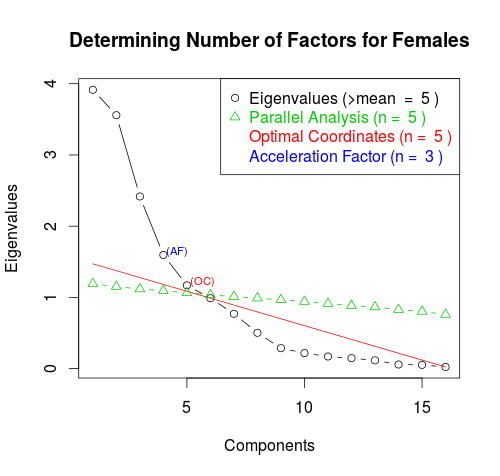
\includegraphics[width = 3.8cm]{graphics/ScreeFem.png}
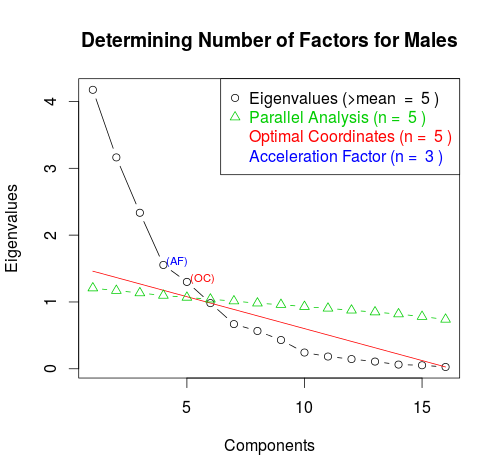
\includegraphics[width = 3.8cm]{graphics/ScreeMale.png}
\caption{{\it Determining Number of Factors}\label{scree}}  
\label{scree}
\end{figure}

Interestingly, although we find that the various factors for male and female speech are similar, they explain different amounts of variation in the data.  For males, the first factor reflects high intensity values and low intensity variation, explaining 18\% of the variation in the male prosodic data.  For females, the fifth and final factor had very similar loadings, only explaining 12\% of the variation in the data.  For females, variation in intensity was one of the most important factors, accounting for 17\% of variation in the data, whereas for males, variation in intensity only accounted for 10\% of the variation in the data.  It may be interesting in the future to investigate how sources of variation in prosody differ across genders and contexts.  

\section{Evaluation Approach}

\subsection{Methodology}
We divide the dataset into two separate groups based on gender. For each gender, we train a classifier for detecting the perception of funny and courteous characteristics.  

We create a training set for a given characteristic for a given gender by splitting the dataset into deciles. We use the top decile as positive and the bottom decile as negative examples. 

\subsection{Classifiers}
We start by using an SVM with a linear kernel. To improve our classifications, we next enforce an L1 norm on the SVM to compensate for the large number of lexical and prosodic features we extract. In case our decision boundaries are non-linear, we also train a RBF kernelized SVM. However, we lose interpretability of the features by using an RBF. So, we train a fourth Adaboost Classifier with decision stumps as weak classifiers to maintain interpretability while also allowing for a non-linear decision boundary. 

\section{Classification Results}
First, we run our four classifiers on our prosodic features only.  Despite only looking at acoustic features of these conversations, we achieve promising results -- an accuracy of 75\% for courteousness and 71\% for funniness.  These results are shown in Table 2.  Interestingly, when attempting prediction from prosody alone, we find that, for male evaluators, prediction based only on the evaluator's speech features outperforms prediction based only on the interlocutor's prosodic features ($p < 0.01$, paired t-test).  This may be because our evaluator \emph{reveals} perceptions of the other person through their prosody.  We do find, however, that the interlocutor's speech is also informative.  In addition, we find that it is far easier to use prosody and lexical features to predict males' evaluation of women than it is to predict women's evaluation of males, as for each classification task, our prediction accuracies are significantly greater than those of the female evaluator counterpart.  

Beyond these two results (that self features are more informative than other features for males and that male evaluators are easier to predict than female evaluators), we may consider that male prosodic features are more informative about our labels than female prosodic features.  We see that with male evaluators, self features are always more informative than other evaluators, but with female evaluators, other features are sometimes more informative. For example, when we predict females' evaluation of males' funniness using the females' lexical features, we achieve an accuracy of only 0.55; however, when we use males' lexical features, we get an accuracy of 0.65.  Here, the males' features are more informative ($p < 0.01$, paired t-test). 

Furthermore, we see that in general prosodic features outperform lexical features, and there is not a huge improvement from independently using prosodic features or lexical features to using both.  This may be due to overfitting in the number of features included -- we note that the L1-penalized SVM improves for the inclusion of more features, even if it is still outperformed by the nonlinear classifiers.  Data reduction, such as that achieved by stacked autoencoders, may be desirable for improved performance from lexical features.
\begin{table*} [t]
\centering
\begin{center}
\vspace{2mm}
\begin{tabular}{c l l l l}
\hline
\multicolumn{1}{l}{\#} & 
\multicolumn{2}{c}{Funny} &
\multicolumn{2}{c}{Courteous}\\
\cmidrule(r){2-3}
\cmidrule(r){4-5}
 & Lexical & Prosodic  & Lexical & Prosodic\\
 \hline
 1 & Other hear & Other imin SD & syllables per turn & imax mean \\
 2 & Other youKnow & Other pslope mean & probably & Other prange mean \\
 3 & Other see & tndur SD & like & Other pmin SD \\
 4 & Other achieve & Other tndur SD & relativ & ptmax SD \\
 5 & Other LaughAcc & Other pslnjmp mean & Other you know & itmin SD \\
 6 & syllables per turn & tndur mean & humans & Other pslnjmp mean \\
 7 & program & pquan mean & cogmech & Other.imin.SD \\
 8 & Other past & imax mean & sad & pquan mean \\
 9 & program & Other tndur mean & Other anxious & ptmin SD \\
 10 & Other pronoun & Other pmax mean & i think & iquan mean \\
 \hline
\end{tabular}
\caption{\label{table:adaboost} {\it  Feature Splits with Highest Weights in Adaboost.}}
\end{center}
\label{table:results}
\end{table*}

\section{Analysis}

By limiting the depth of the trees in Adaboost to 1, we are able to unravel the top features that were used by each tree in Adaboost. We aggregate these top features by summing across the weights associated with each tree split to capture the features with the highest weights.

Since Adaboost learns different classifier each time, we perform a 10 fold feature aggregation and averaging the sum of weights for each feature split. We perform this aggregation by training on lexical and prosodic features independently. Table~\ref{table:adaboost} shows the top features that adaboost splits on. In the table, \textit{Other} refers to the listener's features.

\begin{table*} [t]
\centering
\begin{center}
\vspace{2mm}
\begin{tabular}{c p{5em} p{5em} p{5em} p{5em} p{5em} p{5em} p{5em} p{5em}}
\hline
\multicolumn{1}{l}{\#} & 
\multicolumn{4}{c}{Funny} &
\multicolumn{4}{c}{Courteous}\\
\cmidrule(r){2-5}
\cmidrule(r){6-9}
 & \multicolumn{2}{c}{Lexical} & \multicolumn{2}{c}{Prosodic}  & \multicolumn{2}{c}{Lexical} & \multicolumn{2}{c}{Prosodic}\\
 & Male & Female & Male & Female & Male & Female & Male & Female\\
 \hline
1 & excl & Other LaughAcc & pquan mean & Other tndur SD & syll turn & like & pquan mean & Other prange mean\\
2 & pronoun & Other hear & Other pmean mean & Other imin SD & probably & syll turn & iquan SD & Other pslnjmp mean\\
3 & Other achieve & Other youKnow & Other pquan mean & Other iquan mean & Other anx & Other LaughAcc & Other imin SD & imean SD\\
4 & Other see & kindOf & iquan mean & pquan SD & Other like & Other FuncAcc & imax mean & Other pslope mean\\
5 & achieve & Other program & Other pslope mean & Other pmean SD & aLittle & sad & Other pmin SD & ptmin SD\\
6 & Other youKnow & like & Other imin SD & pmean mean & pronoun & Other youKnow & Other imean SD & ptmax SD\\
7 & Other like & Other iThink & Other prange SD & tndur SD & they & Other friend & imean mean & pquan mean\\
8 & Other you & syll turn & Other pslnjmp mean & pmean SD & humans & relativ & itmin SD & Other imin mean\\
9 & shehe & Other see & tndur mean & Other tndur mean & work & posemo & imin mean & imax SD\\
10 & cogmech & Other affect & imin SD & Other ptmax mean & shehe & Other future & imin SD & imax mean\\
 \hline
\end{tabular}
\caption{\label{table:adaboost} {\it  Gender Based Feature Splits with Highest Weights in Adaboost.}}
\end{center}
\label{table:results}
\end{table*}

\subsection{Funny}
Based on the results for funny, words related the other person using words in the LIWC categories \textit{hear, youKnow, see} and \textit{achieve} are good indicators that the other person finds the speaker funny. The \textit{achieve} category correspond to words like \'win\' that has been expressed by the listener after the speaker delivers a joke. Words corresponding to \textit{hear} and \textit{see} demonstrate that the listener it paying attention and acknowledging the speaker's speech. The 5$^{th}$ feature is laughter accommodation where the listener laughs in reaction to the speaker's laugh.  

The prosodic features for funny also correspond well with the lexical features as shorter \textit{turn duration}, which is the 4$^{th}$ and 5$^{th}$ on the prosodic features list, between the two people usually results in more words in the LIWC \textit{see} and \textit{hear} categories of acknowledgement. These features also show that a high intensity min SD from the listener and a high pitch slope mean are good indicators of funny.

Interestingly, we find that the relevant features vary by gender, as shown in Table 5.  We find that females respond to males varying pitch and intensity, whereas males respond to females with high \emph{average} pitch and high \emph{average} intensity.  In addition, males' own pitch is very important in predicting their evaluations of funniness.  Hedge words are important lexical predictors for both genders.  When males utter many exclamations, they find the female funny.  Females respond to accommodating laughter from their male partners. %HARDCODED TABLE NUMBER

\subsection{Courteous}
Discourse words like \textit{like, probably and I think} are good lexical indicators for detecting courteous. The honesty weakening of there sentences by using such words makes them appear more courteous. Also, talking about \textit{humans} and \textit{cognitive processes} are important. The use of \text{anxious} and \textit{fillers} like \textit{you know} are the only features of the listener that have a high weight.

Low intensity max mean with small pitch range SD and pitch min SD are important prosodic features. This implies that large changes in speech are perceived as non being courteous.

Again, the relevant features vary by gender, as shown in Table 5.  We see that females respond strongly to male accommodation features -- clearly it makes intuitive sense that males with high values for accommodation features will be judged to be more courteous.  Males respond strongly to variation in intensity and pitch from the female, just as they did for funniness.

\subsection{Comparing Funny and Courteous}
It is interesting to note that the speaker's features are the most important when determining whether the speaker will be perceived as courteous. On the other hand, the listeners features are more important for detecting funny.

\section{Future Work}
The model we build has a lot of features and reducing dimensionality of this data by learning hidden variables from an sparse auto-encoder (particularly for the lexical features, as in \cite{ranganath}) might give us more insight into how we can create a shared representation of the lexical with the prosodic features.  In addition, applying simultaneous dimension reduction techniques, such as Canonical Correlations Analysis, across audio, visual and text modes may provide us with interesting insights as to how these media interact. 

We have found here that in general, the evaluator's speech is more informative than the other participant's.  In addition, we have found that, in general, male speech is more informative about males' evaluations of females than female speech is about females' evaluations of men.  In the future, we would like to be able to determine the magnitude of these two effects -- it is difficult to tease apart these effects using the methodologies employed in this paper.

The SpeedDate dataset we use also contains ratings of people's intelligence, sincerity and other characteristics. An interesting area to explore would find correlations between these characteristics and their corresponding prosodic and lexical features.

\section{Conclusion}
In this paper, we evaluate the perceptions of two separate characteristics, funny and courteous, in short meetings like speed dates. Our initial factor analysis of the features show clear distinctions between variations captured amongst males and females. We use different classifiers and obtain a 74\% and 64\% accuracy when predicting funny for males and females respectively. Furthermore, we attain 76\% and 63\% accuracy when predicting courteous. While analyzing the features that correspond to the highest weights in our classifiers, we see a distinct difference between males and females. Models that train using one gender perform better than a model that uses features from both genders. Finally, we see that male prosody tend to be more revealing about their perceptions than female prosody.
%
\eightpt
\bibliographystyle{IEEEtran}
\begin{thebibliography}{10}
\bibitem{ranganath}Ranganath, R., Jurafsky, D., McFarland, D. ``It's Not You, It's Me'', in Proceedings of the 2009 Conference on Empirical Methods in Natural Language Processing.

\bibitem{scherer2003}Scherer, K.R., ``Vocal communication of emotion: a review of research paradigms`` in Speech Communication 40 (1?2), 227?256, 2003

\bibitem{jurafsky}Ranganatha, R., Jurafsky, D., McFarland, D.A., ``Detecting friendly, flirtatious, awkward, and assertive speech in speed-dates``, in Computer Speech \& LanguageVolume 27, Issue 1, Pages 89-115, 2013

\bibitem{ang} Ang, J., Dhillon, R., Krupski, A., Shriberg, E., and Stolcke A.  ''Prosody-based automatic detection of annoyance and frustration in human-computer dialog.'' INTERSPEECH. 2002.

\bibitem{lee} Lee, C., Narayanan, S. and Pieraccini, R. ``Combining acoustic and language information for emotion recognition.'' INTERSPEECH. 2002.

\bibitem{men} Menninghaus, W., Bohrn, I., and Altmann, U.  ''Sounds funny? Humor effects of phonological and prosodic figures of speech.'' Psychology of Aesthetics, Creativity, and the Arts 8.1 (2014): 71.

\bibitem{pur} Purandare, A., and Litman, D. ''Humor: Prosody analysis and automatic recognition for f* r* i* e* n* d* s*.'' Proceedings of the 2006 Conference on Empirical Methods in Natural Language Processing. Association for Computational Linguistics, 2006.

\bibitem{fein} Feinberg, David R., Jones, B. Little, A., D. Michael Burt, and Perrett, D. 2005. ''Manipulations of Fundamental and Formant Frequencies In�uence the Attractiveness of Human Male Voices.'' Animal Behaviour 69 pp: 561-568.

\bibitem{Mair} Mairesse, F., Walker, M., Mehl, M., and Moore, K. ''Using Linguistic Cues for the Automatic Recognition of Personality in Conversation and Text.'' J. Artif. Intell. Res.(JAIR) 30 (2007): 457-500. 

\bibitem{Grav} Gravano, A., Levitan, R., Willson, L., Benus, S., Hirschberg, J., Nenkova, A. ``Acoustic and prosodic correlates of social behavior.`` 2011

\bibitem{pennebaker}Pennebaker, J. W., Booth, R., Francis, M., ``Linguistic inquiry and word count: LIWC2007`` ? operator�s manual. Tech. rep., University of Texas, 2007

\bibitem{natale}Natale, M.,  ``Convergence of mean vocal intensity in dyadic communication as a function of social desirability``, in Journal of Personality and
Social Psychology 32 (5), 790-804, 1975

\bibitem{ireland}Ireland, M.E., Slatcher, R.B., Eastwick, P.W., Scissors, L.E., Finkel, E.J., Pennebaker, J.W., ``Language style matching predicts relationship initiation and stability``, in Psychological Science 22 (1), 39, 2011

\bibitem{levitan}Levitan, R., Hirschberg, J., ``Measuring acoustic-prosodic entrainment with respect to multiple levels and dimensions``, in ACL 2011

\bibitem{hay} Hayton, J., Allen, D., and Scarpello, V.. ``Factor retention decisions in exploratory factor analysis: A tutorial on parallel analysis`` in Organizational research methods 7.2: 191-205, 2004
\end{thebibliography}
\end{document}
